\section{Motivation and Background}
\label{sec:motivation}

In high performance computing (HPC), maximizing performance is the main
objective. However, in order to reach extreme scale computing, it is necessary
to also improve the energy efficiency of current applications and algorithms.
This section explains why approximate computing is potential solution and why
MG solvers are a good candidate for this type of optimizations.

\subsection{Approximate Computing}
\label{sec:approx}

%\leo{A very brief introduction to approximate computing.. }
%\marc{

Approximate computing categorizes a wide set of techniques aimed at trading off computation's quality with cost.
It is based on the intuition that operating at peak level accuracy may produce significant resource waste without adding any valuable information to the numerical data.
The increasing restrictions that parallel architectures are suffering in terms of power and circuitry area have made the approximate computing field an appealing and cost-effective approach that can be potentially applied to a wide range of application domains like data analytics, scientific computing, multimedia or signal
processing~\cite{Mittal2016}.
Indeed, recent approaches demonstrate how up to 50x enery savings can be achieved when applying approximate computations to the k-means clustering algorithm while only losing 5\% classificatin accuracy~\cite{Chippa2013}.
Also, an approximate approach based on neural networks can speedup an inverse kinematics application by more than 20x by allowing a final application error of just 5\%~\cite{Grigorian2015}.

Despite its potential, approximate computing must be applied in an extremely careful way.
For example, reducing the accuracy of control flow instructions or memory addresses computations may cause segmentation faults.
Also, applying approximate techniques to floating point computations can potentially bring wrong results or cause iterative algorithms to stall if they are blindly applied.
The success of approximate approaches requires them to be judicisouly applied to the most low-accuracy tolerant phases of numerical algorithms.
In this paper we apply approximate computing approaches to the MG solver in several different ways.
Some of them reduce the amount of computations of certain routines while keep the accuracy of each computation, like reducing on the number of relaxation iterations (Section~\ref{sec:pruning}).
Other approaches keep the number of computations but reduce their accuracy, like using floating point representations with less bits devoted to store the mantissa (Section~\ref{sec:precision}).

 


%}

\begin{figure}[hbt]
 \resizebox{\linewidth}{!}{
    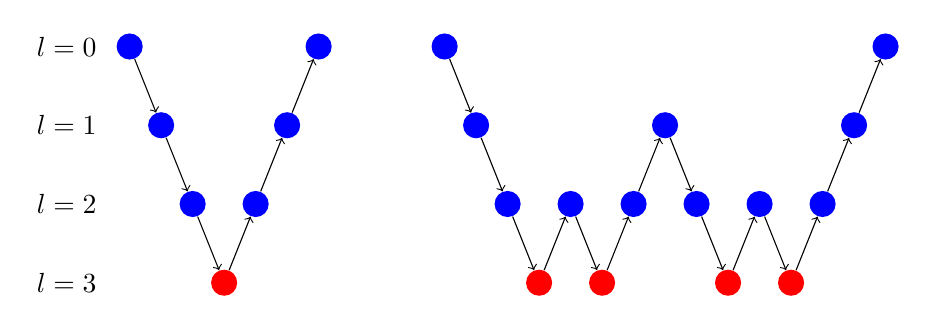
\begin{tikzpicture}

 \begin{scope}[xscale=2/5]

  \node (sh) at (-5,3) { $l=0$ };
  \node (shh) at (-5,2) { $l=1$ };
  \node (shhh) at (-5,1) { $l=2$ };
  \node (shhhh) at (-5,0) { $l=3$};

  %\node (title) at (0,5) { V-cycle k=1};
  %\node (title2) at (14,5) {W-cycle k=2};

    \node[circle,fill=blue] (a) at (-3,3) { };
    \node[circle,fill=blue] (b) at (-2,2) {};
    \node[circle,fill=blue] (c) at (-1,1) {};
    \node[circle,fill=red] (d) at (0,0) {};
    \node[circle,fill=blue] (e) at (1,1) {};
    \node[circle,fill=blue] (f) at (2,2) {};
    \node[circle,fill=blue] (g) at (3,3) {};

    \draw[->] (a) -- (b);
    \draw[->] (b) -- (c);
    \draw[->] (c) -- (d);
    \draw[->] (d) -- (e);
    \draw[->] (e) -- (f);
    \draw[->] (f) -- (g);

    \node[circle,fill=blue] (aa) at (7,3) { };
    \node[circle,fill=blue] (ab) at (8,2) {};
    \node[circle,fill=blue] (ac) at (9,1) {};
    \node[circle,fill=red] (ad) at (10,0) {};
    \node[circle,fill=blue] (ae) at (11,1) {};
    \node[circle,fill=red] (af) at (12,0) {};
    \node[circle,fill=blue] (ag) at (13,1) {};
    \node[circle,fill=blue] (ah) at (14,2) {};
    \node[circle,fill=blue] (ai) at (15,1) {};
    \node[circle,fill=red] (aj) at (16,0) {};
    \node[circle,fill=blue] (ak) at (17,1) {};
    \node[circle,fill=red] (al) at (18,0) {};
    \node[circle,fill=blue] (am) at (19,1) {};
    \node[circle,fill=blue] (an) at (20,2) {};
    \node[circle,fill=blue] (ao) at (21,3) {};

    \draw[->] (aa) -- (ab);
    \draw[->] (ab) -- (ac);
    \draw[->] (ac) -- (ad);
    \draw[->] (ad) -- (ae);
    \draw[->] (ae) -- (af);
    \draw[->] (af) -- (ag);
    \draw[->] (ag) -- (ah);
    \draw[->] (ah) -- (ai);
    \draw[->] (ai) -- (aj);
    \draw[->] (aj) -- (ak);
    \draw[->] (ak) -- (al);
    \draw[->] (al) -- (am);
    \draw[->] (am) -- (an);
    \draw[->] (an) -- (ao);

 \end{scope}

\end{tikzpicture}


 }
 \caption{V-cycle and W-cycle on 4-level grid.}
 \label{fig.cycles}
\end{figure}

\subsection{Multi-Grid Algorithm}
\label{sec:algo}

MG's cycles start and end on the finest grained grid and are defined by the
order in which its different coarseness levels are applied.  The simplest cycle
is the V-cycle, already described in Section~\ref{sec:intro}, where a few
iterations of an iterative method (the \textit{Relaxation} step) is performed
at each level from the finest to the coarsest level and then in the reverse
order.  Another common approach is the W-cycle scheme where the coarsest grid
level is reached several times before going back to the finest grid level.  It is
possible to generalize the notion of cycle to a $k$-cycle (where a V-cycle is a
$1$-cycle and a W-cycle is a $2$-cycle).  Figure~\ref{fig.cycles} shows a
representation of the V- and the W-cyles with 4 levels where we can see how the
W-scheme goes back and forth the coarsest level 4 times before reaching again
the finest level of the grid.  The cycles are executed multiple times
iteratively until the error is lower or equal to a certain \emph{tolerance}
(i.e., the expected accuracy) or until the maximum number of cycles is reached.

%\subsection{Definitions}

%\begin{itemize}
% \item A system of equations is represented by the following equation: $Ax=b$, where $A \in \mathcal{M}(\mathbb{R})^{n\times n}$ and $b \in \mathcal{\mathbb{R}}^n$ are given and
% $x \in \mathbb{R}^n$ is the unknown. The \emph{exact} solution of this system will be denoted by $\widetilde{x}$.
% \item A level is an integer between $1$ and $L$. Level $1$ will be called the finest level, and level $L$ will be called the coarsest level.
%  \item The restriction of $A$ (or $b$ or $x$) to level $l$ will be denoted by $A^l$ (or $b^l$ or $x^l$). We have $A^1 = A$ (and $b^1=b,x^1=x$).
%  \item We define a set of $L-1$ restriction matrices $R_1,\dots,R_{L-1}$ such that $R_l b^l = b^{l+1}$. We also define some prolongation matrices $P_1,\dots,P_{L-1}$ such that $P_{l}b^{l+1} = b^l$.
%  In other words, we have $P_l = {R_l}^{-1}$ (left inverse) and we build the $A^l$ matrices as follows: $A^{l+1} = R_l A^l P_l$.
%  \item We denote by $e^l$ the error at level $l$, that is the vector such that $x^l + e^l = \widetilde{x^l}$, that is to say $\widetilde{x^l}-x^l$.
%  We also define the residual at level $l$, $r^l = b^l - A^lx^l$. As $b^l = A^l\widetilde{x^l}$, we can also write $r^l = A^le^l$.
%  \item We derive the relative residual norm at any step $i$ in the algorithm
%  by the norm of the residual at this step, $||b^l - A^lx^l_i||$, divided by the norm of the initial residual, $|| b^l - A^lx^l_0||$.\\ We also define the notion of \emph{tolerance}
%  as an real value between 0 and 1, which is a threshold for stopping an algorithm. In multi-grid algorithms, this threshold will be on the residual norm.
%  \item We call relaxation a step of an iterative method for solving linear systems (such as Jacobi, Gauss-Sneidel, \dots). Formally, for a vector $x \in \mathbb{R}^n$, it represents the computation of
%  $x \leftarrow Mx + c$ where $M \in \mathcal{M}(\mathbb{R})^{n\times n}$ and $c \in \mathcal{\mathbb{R}}^n$ are defined depending on the method used.
% \end{itemize}

%\subsection{The V-cycle}

%  The goal of the algorithm is to improve the efficiency of iterative methods.
%  Indeed, the choice of the starting vector $x$ on which to apply relaxations
%  has consequences on the convergence time of the solver, and depending on the
%  system to solve, the factor of convergence (related to the matrix $M$) can
%  be close to 1.\\ Here the idea is to do some relaxations and then correct
%  the value of $x$ by adding to it the corresponding error term. However, this
%  error term cannot be computed easily (otherwise, solving the problem would
%  be done by computing the error term and adding it to $x$). Multi-grid
%  solvers instead use recursion to compute the error term. The stopping
%  parameter for the recursion will be determined by decreasing the sizes of
%  vectors and matrices (thus loosing some accuracy but saving time).
%  Formally, we can sum up the algorithm as follows:


%  MG$(l,x,f,\alpha_1,\alpha_2)$:
%  \begin{itemize}
%    \item If $l = L$, return $x = {A^L}^{-1} f$ (exact solve);
%    \item Else:
%    \begin{enumerate}
%      \item Relax $x$ $\alpha_1$ times using an iterative method (matrix $A^l$, right hand side $f$);
%      \item $r \leftarrow R_l ( f - Ax )$;
%      \item $y \leftarrow 0$:
%      \item MG$(l+1,y,r,\alpha_1,\alpha_2)$;
%      \item $e \leftarrow P_{l} y$;
%      \item $x \leftarrow x+e$;
%      \item Relax $x$ $\alpha_2$ times using an iterative method (matrix $A^l$, right hand side $f$);
%   \end{enumerate}
%  \end{itemize}
%  The algorithm is then executed by setting $x^l \leftarrow 0$ and then executing MG$(1,x^l,b^l,\alpha_1,\alpha_2)$.
%
%  Then several ways of modifying the algorithm appear:
%  \begin{itemize}
%   \item Which iterative method to use?
%   \item Do we want only one recursive call at each level or more?
%   \item How many times do we need to apply the algorithm?
%   \item How to determine good $\alpha_1$ and $\alpha_2$ parameters?
%   \item How many levels should be defined?
%  \end{itemize}
%
%  In all what follows the iterative method chosen is an hybrid
%  Jacobi/Gauss-Seidel method. The number of levels used will not be studied.



